\section{Predator-Prey}

\begin{frame}
\begin{center}
    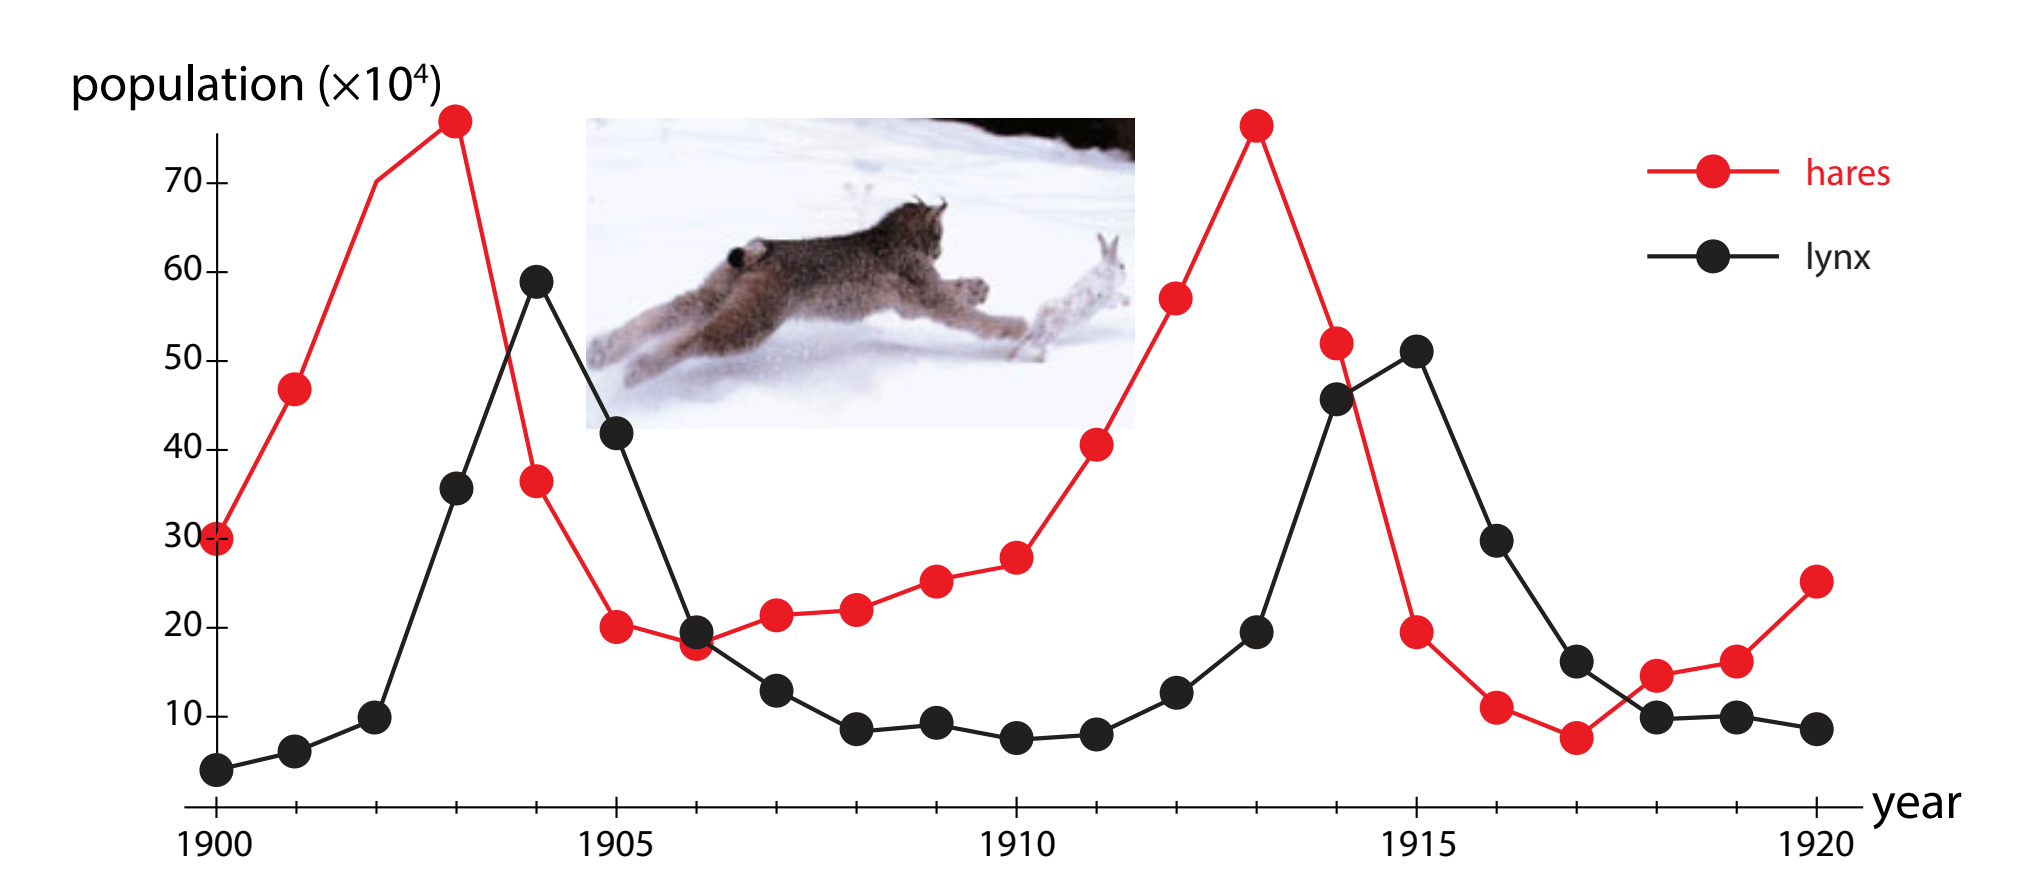
\includegraphics[scale=0.25]{lesson_2/images/predator_plot.png}
\end{center}
    
\end{frame}

\begin{frame}
    \frametitle{Overview}
    \begin{itemize}
        \item The Lotka-Volterra equations, also known as the predator-prey equations, model the dynamics of biological systems in which two species interact, one as a \textbf{predator} and the other as \textbf{prey}.
        \item They were proposed independently by Alfred J. Lotka in 1925 and Vito Volterra in 1926.
        \item   Model is characterized by \textbf{oscillations} in the population size of both predator and prey,
        \item Peak of the predator's oscillation lags  behind the peak of the prey's oscillation.
    \end{itemize}
\end{frame}

\begin{frame}{Assumptions}
         The model makes several simplifying assumptions but captures the essential dynamics of predator-prey interactions:
        \begin{itemize}
         \pause
          \item  the prey population will grow exponentially when the predator is absent (unrealistic in a long term but may be precise for a long period) 
           \pause
          \item the predator population will starve in the absence of the prey population --- there is no option of  switching to another type of prey (may be realistic for some circumstances) 
           \pause
          \item predators can consume any quantities of prey (unrealistic for large quantities)
           \pause
          \item both populations are moving randomly through a homogeneous, static, environment (may be approximately true for some environments)
        \end{itemize}

\end{frame}

\begin{frame}{The Mathematical Model}
\small
    The Lotka-Volterra equations are a pair of first-order, nonlinear, differential equations given by:
    \begin{equation}
        \frac{dN}{dt} = rN - \beta NP
    \end{equation}
      \begin{equation}
        \frac{dP}{dt} = m\beta NP - dP
    \end{equation}
    \pause
    where:
    \begin{itemize}
        \item $N$ is population number of prey (e.g., rabbits),
            \pause
        \item $P$ is the number of predators (e.g., foxes),
        \item $r$ is the prey growth rate
            \pause
        \item $d$ is the death rate of predators
            \pause
        \item $m$ is the proportionality constant
            \pause
        \item $\beta$ attack efficiency of the predator
    \end{itemize}
\end{frame}


\begin{frame}{Prey equations}
\footnotesize
    The prey population is given by:
    \begin{equation}
        \frac{dN}{dt} = rN - \beta NP
    \end{equation}
    
    \pause
    In the absence of predators, the equation becomes:
    \begin{equation}
        \frac{dN}{dt} = rN 
    \end{equation}
    which represents the Malthusian model. The prey population would grow exponentially with the growth rate $r$.

    \pause
 \vfill{1em}
    The reduction in prey population due to predators is captured by the expression:
    \begin{equation}
        - \beta NP
    \end{equation}
    \pause
    Here, $NP$ is proportional to the number of encounters. An increased number of predators, an increased prey population, and greater searching efficiency of the predators would all lead to a higher removal rate of prey.
    $\beta$ is attack efficiency of the predator. Higher $\beta$ means higher probability of prey being killed.
\end{frame}


\begin{frame}{Predator-prey encounters}
Picture below illustrates the concept of predators-prey encounters as $N \cdot P$ product.
\vfill
\begin{center}
     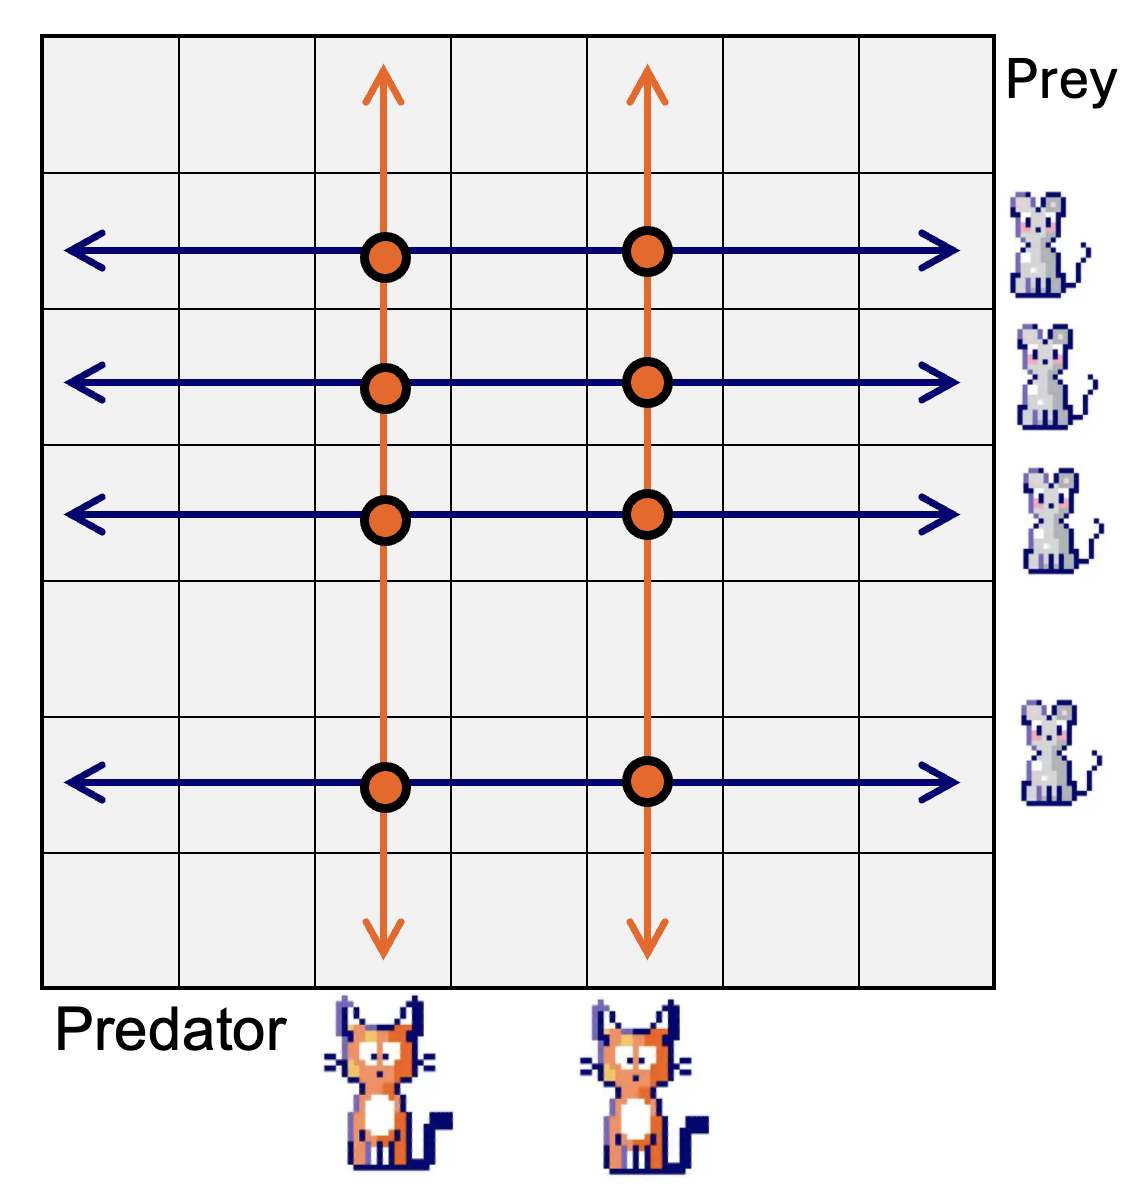
\includegraphics[scale = 0.22]{lesson_2/images/predator_meetings.png}
\end{center}
\pause
The concept would not work for predators hunting in packs or for  prey staying in herds. 
\end{frame}

\begin{frame}{Predator equations}
\footnotesize
    The predator population is given by:
      \begin{equation}
        \frac{dP}{dt} = m\beta NP - dP
    \end{equation}
    \pause
    If the prey population $N$ is 0, the equation becomes:
    \begin{equation}
        \frac{dN}{dt} = - dN 
    \end{equation}
    which represents dying of prey at exponential rate $d$.

\vfill
     \pause
    The growth of predator population growth by eating of prey
    \begin{equation}
        + m \beta NP
    \end{equation}
    Here we see again $\beta NP$. Proportionality constant $m$ tells how many prey individuals are required for increase of predator population by one. 
\end{frame}


\begin{frame}
\begin{center}
    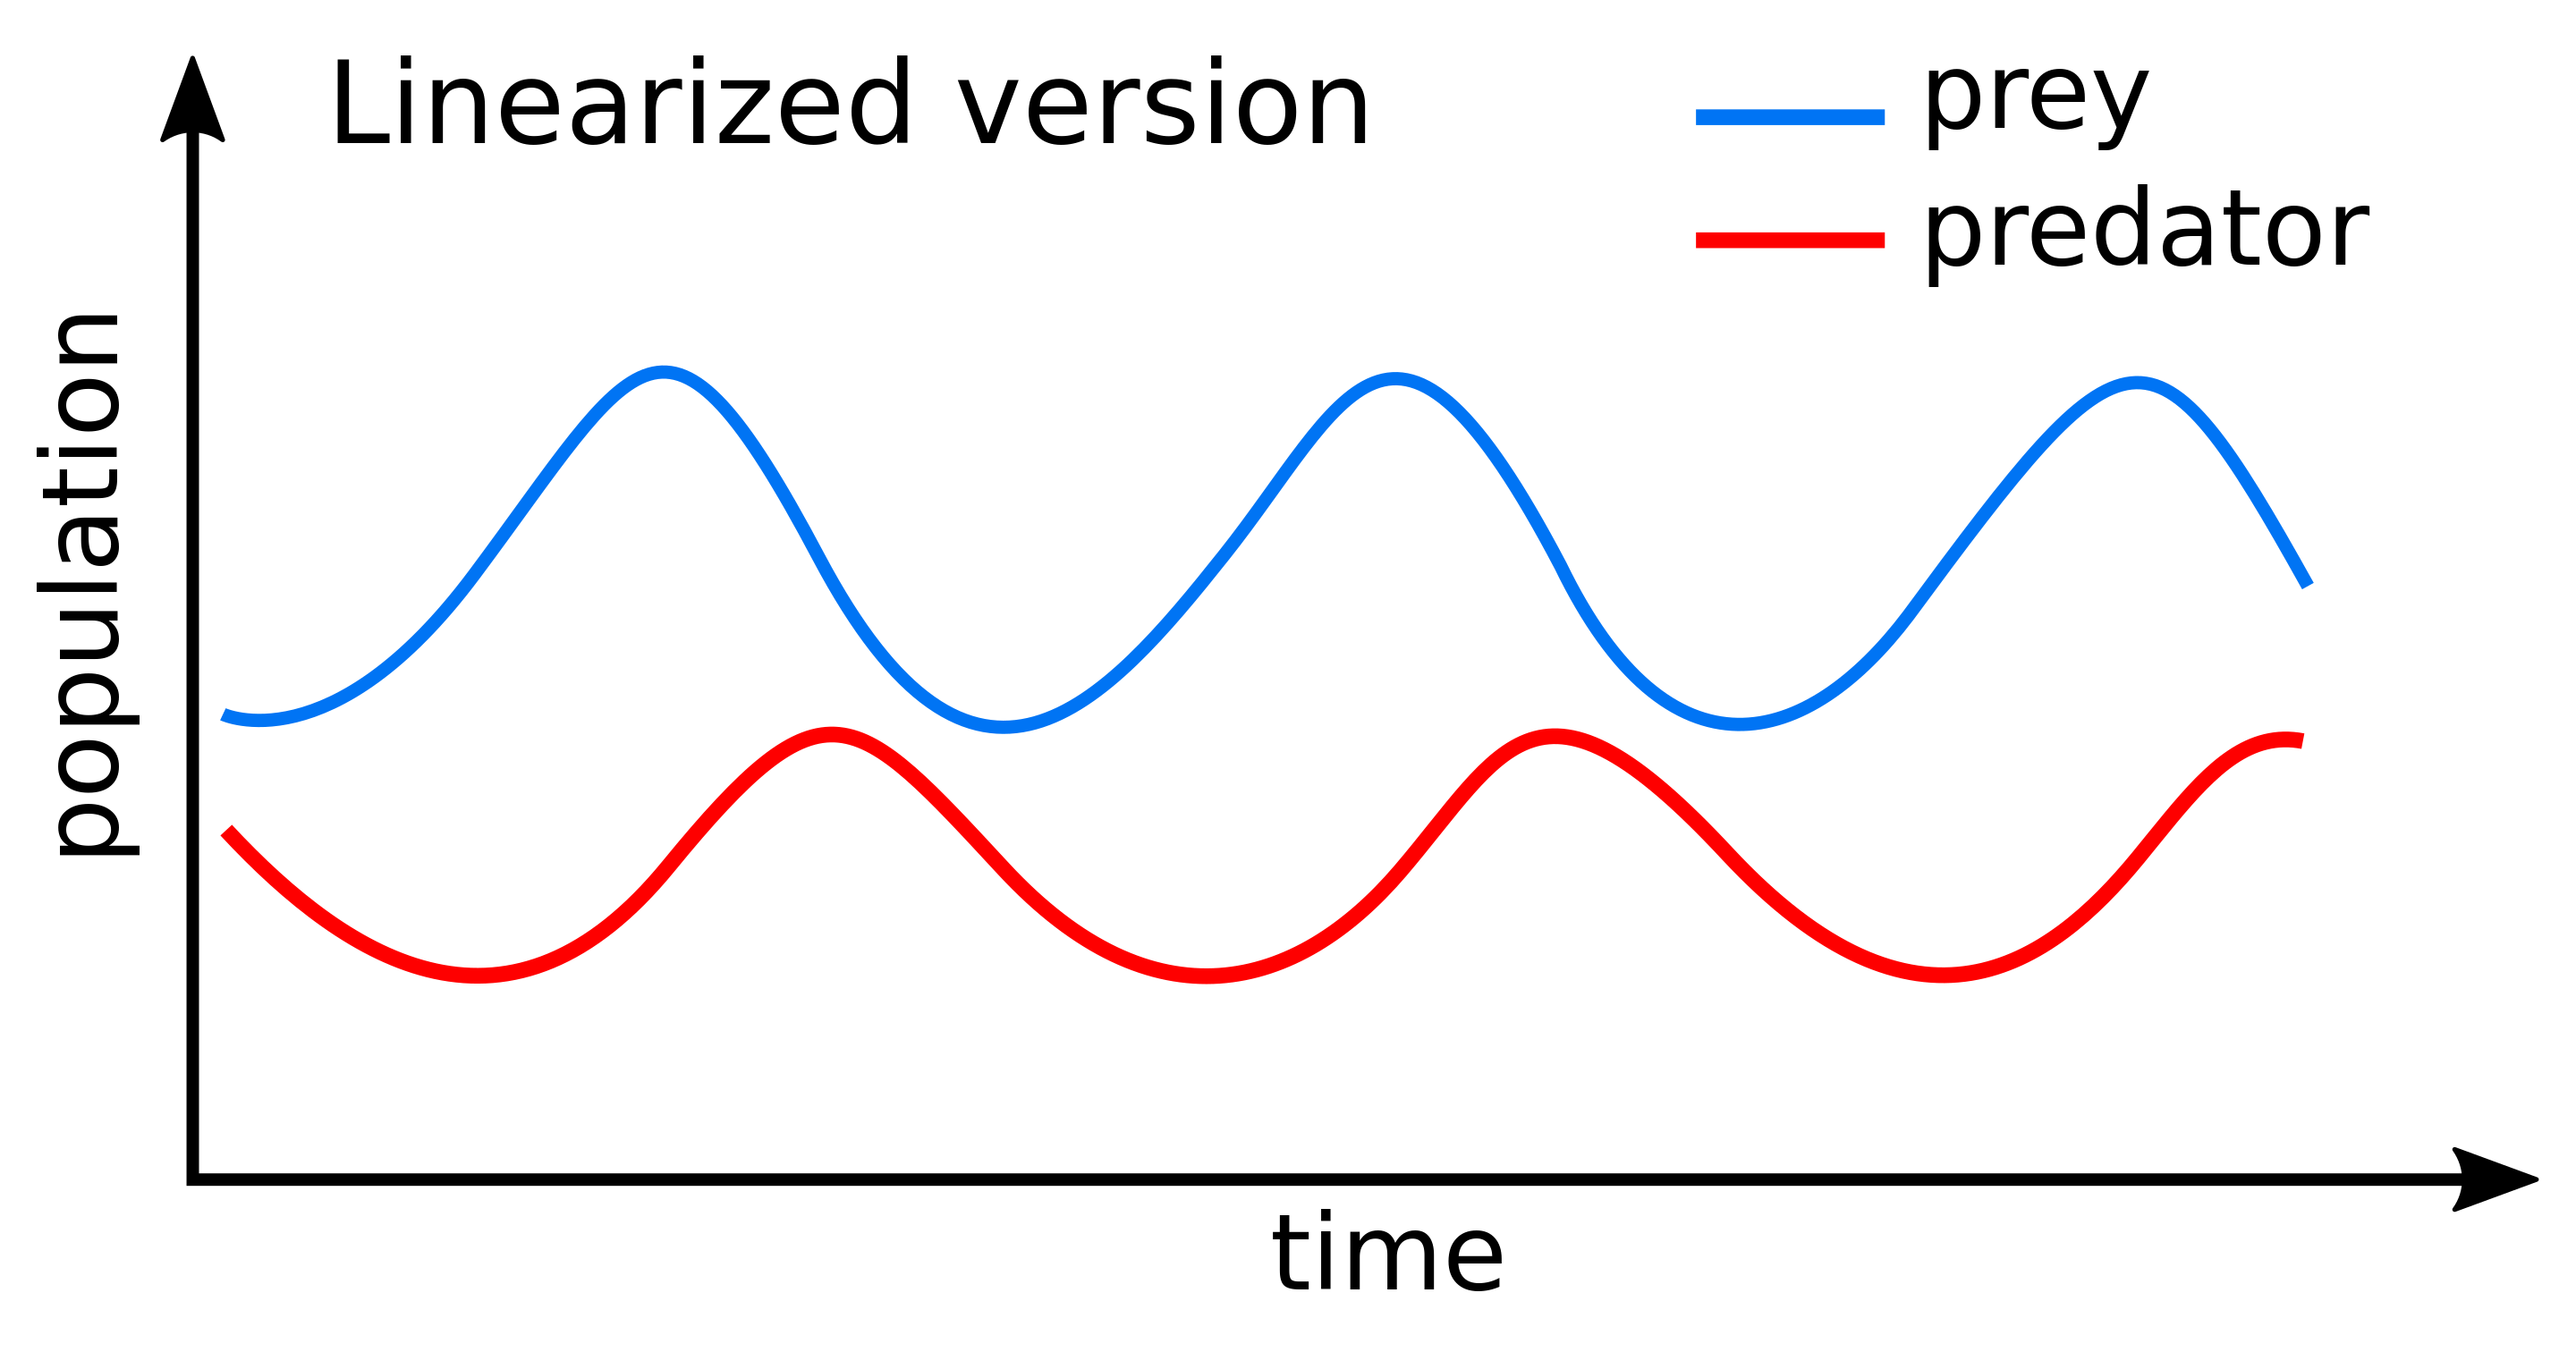
\includegraphics[scale = 0.1]{lesson_2/images/predator_prey_in_time.png}
\end{center}
    
\end{frame}

\begin{frame}
\begin{center}
     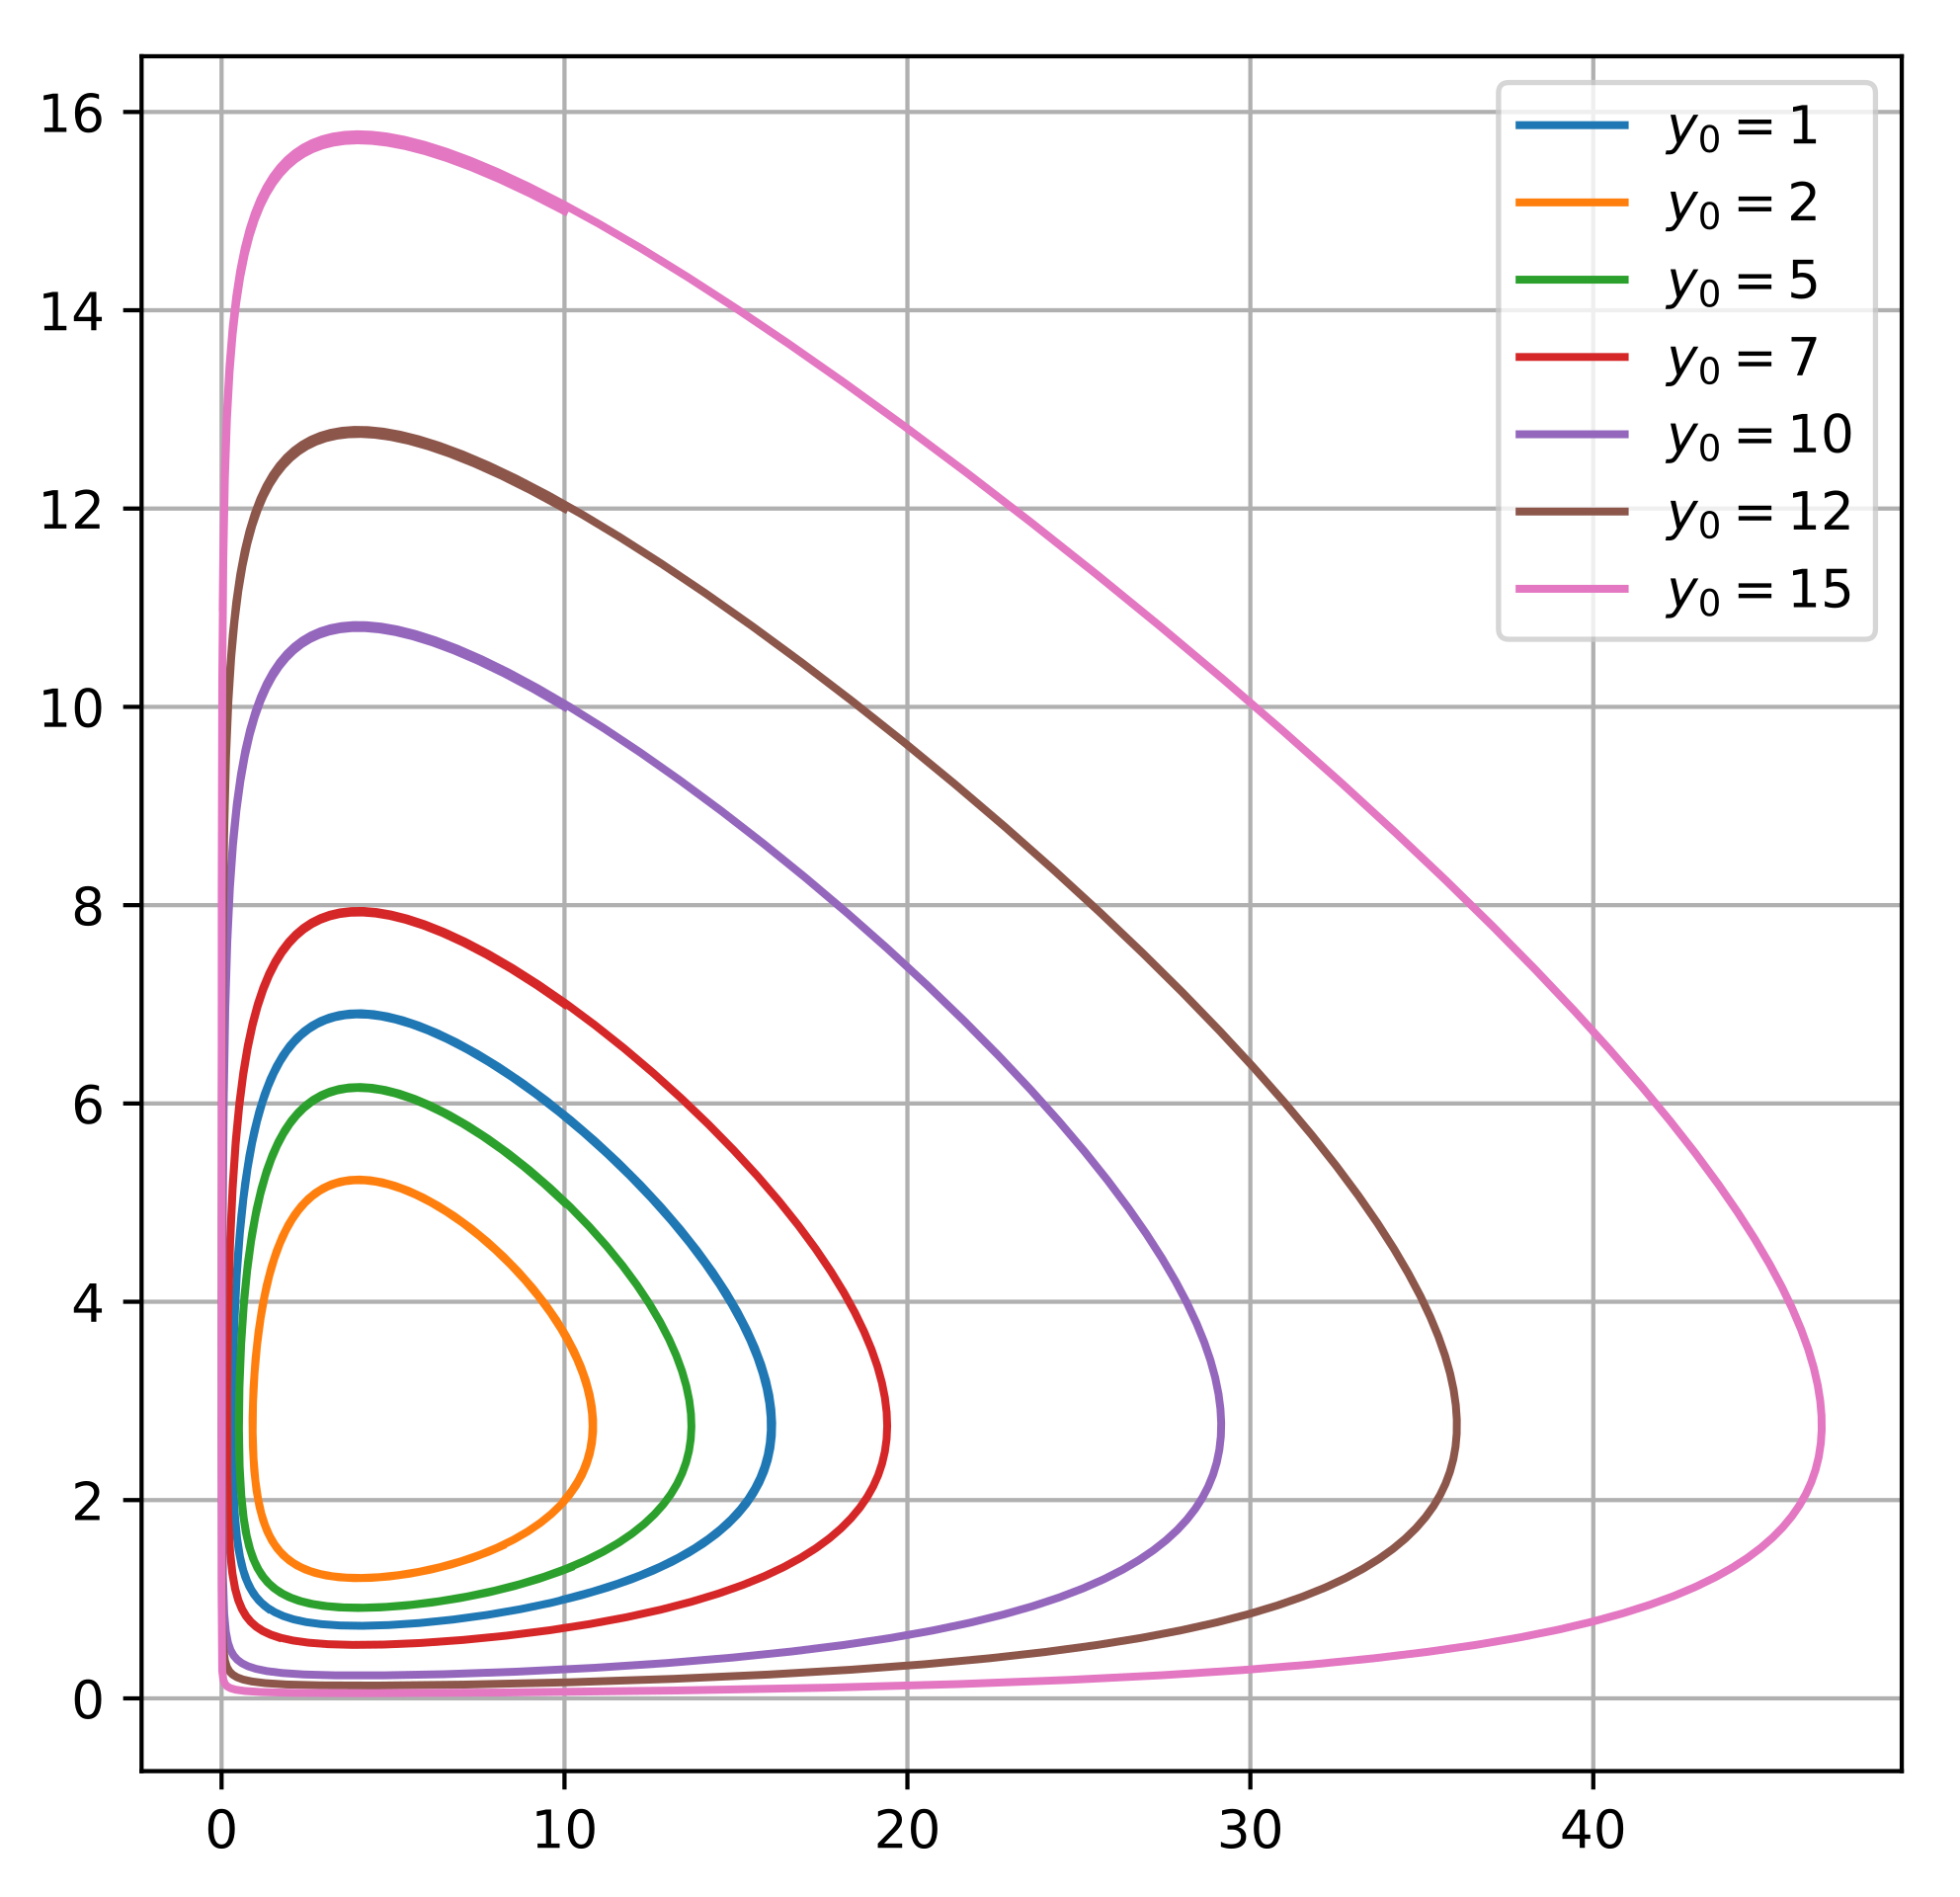
\includegraphics[scale = 0.1]{lesson_2/images/predator_prey_space.png}
\end{center}
   
\end{frame}

\begin{frame}{Concept of feedback}
\begin{center}
    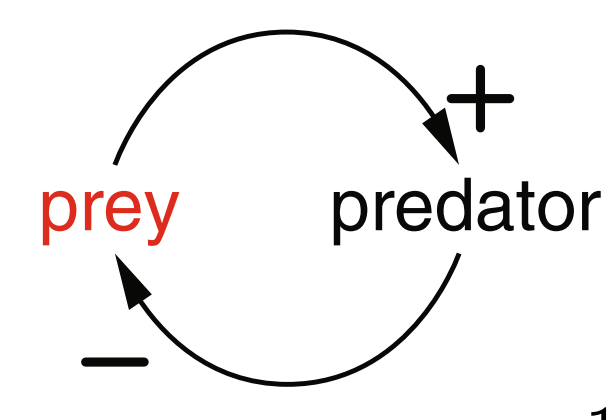
\includegraphics[scale = 0.5]{lesson_2/images/predator_feedback.png}
\end{center}
    
\end{frame}

\begin{frame}
    \frametitle{Biological Implications}
    \begin{itemize}
        \item The model predicts oscillations in the populations of predator and prey.
        \item The fluctuation of the two species is periodic,
    \item The amplitude and period of these oscillations depend on the initial conditions and the parameters of the model.
    \item  The \textit{average} numbers of the two species are constant
    \item  If we  destroy individuals of both species  proportionately to their number, the average number of individuals of the prey grows and the average number of predators diminishes.
    \end{itemize}
\end{frame}


\begin{frame}
    \frametitle{Conclusion}
    \begin{itemize}
        \item The Lotka-Volterra predator-prey model provides a  framework for understanding the dynamics of biological systems with predator-prey interactions.
        \item Despite its simplicity, it offers valuable insights into the oscillatory nature of ecological populations and has motivates further research into more complex and realistic models.
    \end{itemize}
\end{frame}

\begin{frame}{Exercise: Building a Predator-Prey Model in Simulink}
\small

        Use Simulink to construct and analyze the Lotka-Volterra model.


        \begin{enumerate}
        \footnotesize
            \item Create a new Simulink model and build the system using two integrator blocks representing the populations of predators and prey.
            \item Use function blocks to implement the differential equations for each population.
            \item Set initial populations for predators and prey using constant blocks.
        \end{enumerate}
        Experiment with the following parameters and observe the effects on the population dynamics. 
 \begin{enumerate}
     \footnotesize
            \item Adjust the prey growth rate $r$ to see how it affects the population cycles.
            \item Study the impact the predator death rate $d$)
            \item Modify the attack efficiency $\beta$ and observe the changes in the frequency and amplitude of the oscillations.
            \item Experiment with the conversion efficiency $m$
             \end{enumerate}

    Plot predator and prey population in time and phase-space plot for the predator prey system.

\end{frame}

